\chapter{Background}\label{ch:background}
In this chapter we provide the background needed for different concepts that are discussed in this thesis. In section \ref{sec:cnn} we introduce convolutional neural networks and how they are trained. Moreover we define the necessary terminology and provide the mathematical background required to navigate this thesis. Section \ref{sec:synth} provides the terminology that we use throughout this thesis to describe small parts, synthetic images and real images.


\section{Convolutional Neural Networks}\label{sec:cnn}
A \textbf{neural network} is a massively parallel distributed processor made up of single processing units, which has a natural propensity for storing experiential knowledge and making it available for use \cite{haykin1994neural}. Convolutional neural networks are a special type of neural network. They are typically used to solve computer vision problems like image classification and object recognition.

Regular neural networks consist of an \textbf{input layer}, \textbf{hidden layers} and an \textbf{output layer}. Every layer is made up of a set of \textbf{neurons}, where each neuron is fully connected to all neurons in the layer before. A neuron which has an input $x$ of size $n$ calculates the weighted sum $z$ as follows: \[ z = \sum_{i=1}^n w_ix_i + b_i \] where $w$ is called \textbf{weight} and $b$ is called \textbf{bias}. The weights and biases of all the neurons in a network are called the network \textbf{parameters}. Each neuron calculates its ouput $y$ by applying a differentiable non-linear function $\varphi(\cdot)$, called the \textbf{activation function}, to the weighted sum of its input signals $z$. \[y = \varphi(z)\] A neural networks relays the output of its neurons through a series of hidden layers. Finally, the last fully-connected layer, called the output layer, computes the predictions of the neural network. Figure \ref{fig:NN} shows an example structure of a regular neural network.

\begin{figure}[H]
\centering
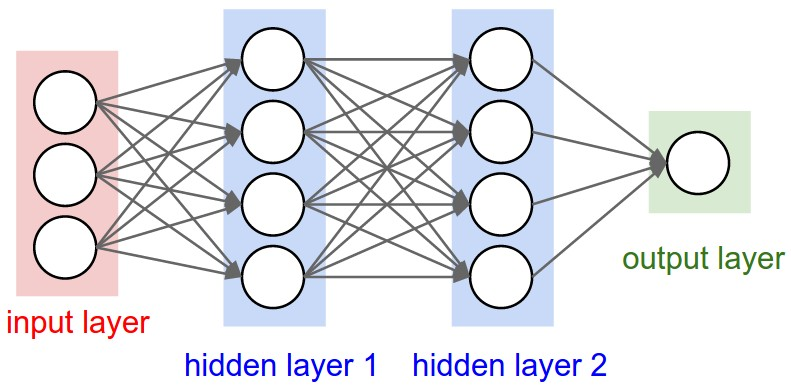
\includegraphics[width=0.75\textwidth]{NN}
\caption[A neural network with an input layer, two hidden layers and an ouput layer. Each neuron is fully connected to all the neurons in the preceeding layer.]{A neural network with an input layer, two hidden layers and an ouput layer. Each neuron is fully connected to all the neurons in the preceeding layer.\footnotemark}
\label{fig:NN}
\end{figure}
\footnotetext{Image: http://cs231n.github.io/convolutional-networks/}

Convolutional neural networks (CNNs) are structured differently. CNNs have 3 types of layers: \textbf{convolution layers}, \textbf{pooling layers} and \textbf{fully connected} layers. Convolution layers slide a weighted matrix (called \textbf{filter} or \textbf{kernel}) over the previous layer, and calculate the sum of products. The size of the step that the filter takes while sliding is called a \textbf{stride}. Figure \ref{fig:CONV} shows how a convolution layer applies a 3x3 filter to the previous layer. A non-linear activation function is applied to the output of the convolution operation to create a \textbf{feature map}. It is common to add a pooling layer after the convolution layer for subsampling, which reduces the convolution layer dimentionality. A frequently used type of pooling is \textbf{max pooling} \cite{weng1992cresceptron}. Max pooling divides the input layer into sections and computes the maximum activation of each section. Figure \ref{fig:MP} shows how a max pooling layer applies a 2x2 filter to the preceding layer. Fully connected layers are similar to layers in a regular neural network. Each neuron in a fully connected layer is connected to all neurons in the previous layer.

Figure \ref{fig:lenet5} shows the Lenet-5 convolutional neural network, which was designed by LeCun et al. \cite{lecun1998gradient} for handwritten digit recognition. Lenet-5 is an example of a CNN \textbf{architecture}. A CNN architecture is a set up of different types of layers which are combined to predict the class of the input image.

\begin{figure}[H]
\centering
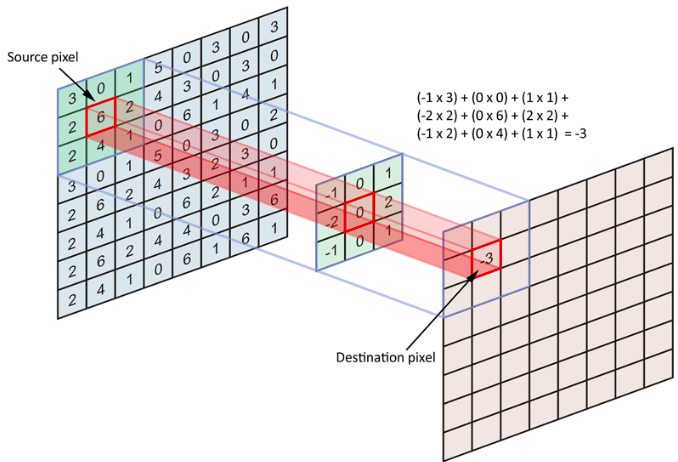
\includegraphics[width=\textwidth]{CONV}
\caption[A 3x3 filter is applied to the source pixel. Each weight in the filter is multiplied by the source's neighbouring pixel in the corresponding position. The sum of products is used to calculate the destination pixel's value in the output feature map.]{A 3x3 filter is applied to the source pixel. Each weight in the filter is multiplied by the source's neighbouring pixel in the corresponding position. The sum of products is used to calculate the destination pixel's value in the output feature map.\footnotemark}
\label{fig:CONV}
\end{figure}
\footnotetext{Image: https://towardsdatascience.com/applied-deep-learning-part-4-convolutional-neural-networks-584bc134c1e2}

\begin{figure}[H]
\centering
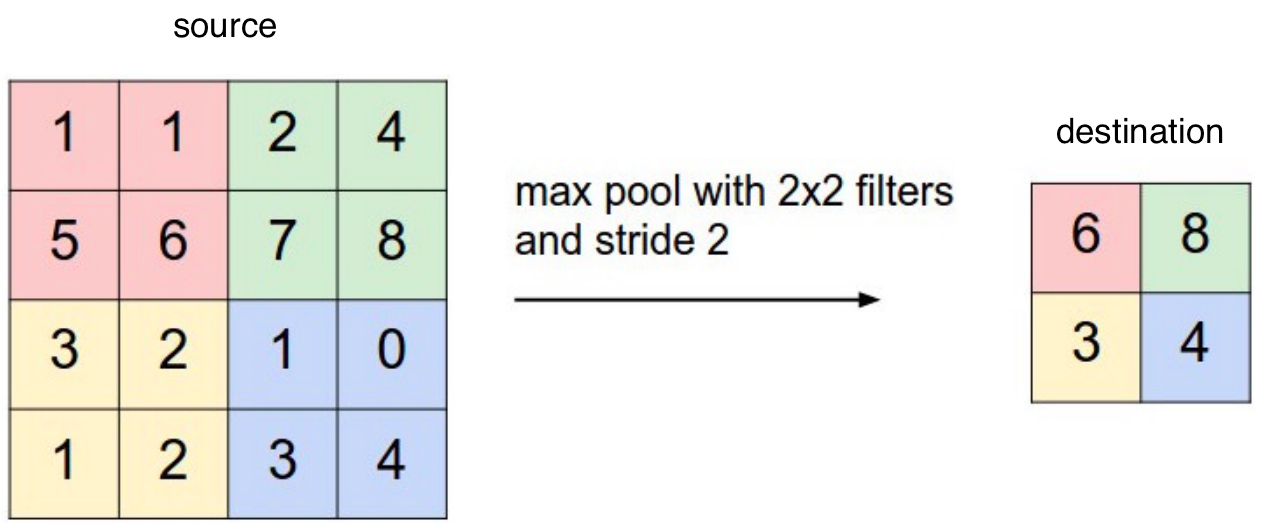
\includegraphics[width=0.7\textwidth]{MP}
\caption[A max-pooling filter of size 2x2 and stride 2 is applied to the source feature map. The maximum value of each filter is used in the destination feature map.]{A max-pooling filter of size 2x2 and stride 2 is applied to the source feature map. The maximum value of each filter is used in the destination feature map.\footnotemark}
\label{fig:MP}
\end{figure}
\footnotetext{Image: http://cs231n.github.io/convolutional-networks/}

\begin{figure}[H]
\centering
\makebox[\textwidth][c]{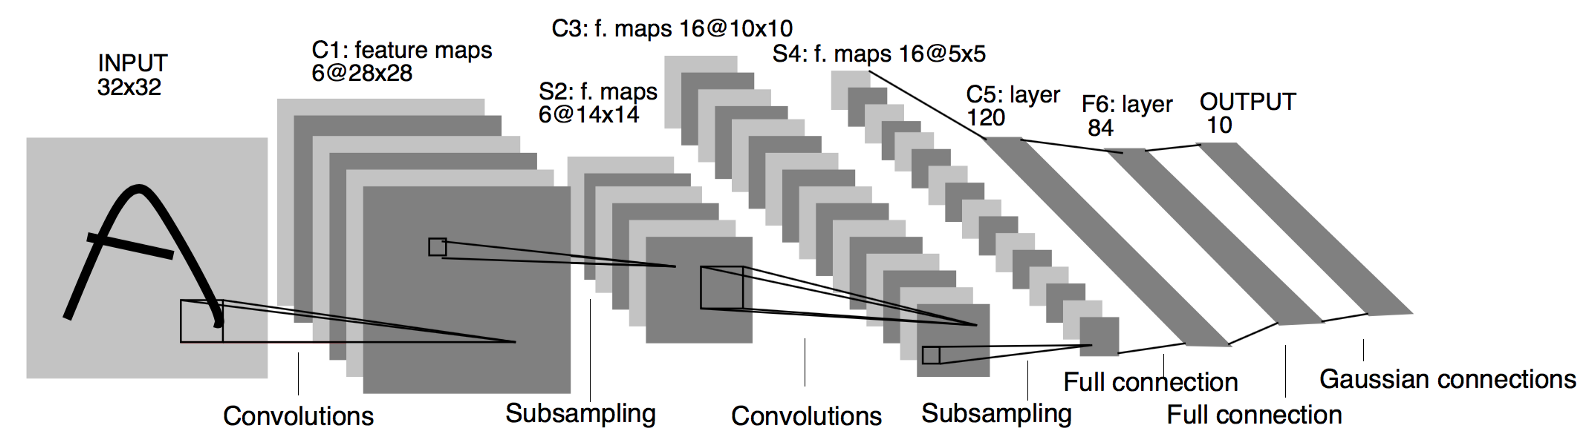
\includegraphics[width=1.3\textwidth]{lenet5}}
\caption[Architecture of the Lenet-5 convolutional neural network.]{Architecture of the Lenet-5 convolutional neural network.\cite{lecun1989backpropagation}}
\label{fig:lenet5}
\end{figure}

The Lenet-5 network uses 3x3 filters with a stride of 1 for convolution layers and 2x2 filters with a stride of 2 for subsampling layers. Lenet-5 uses \textbf{average pooling}, which calculates the average of the values in the filter.

The network takes a 32x32 image as input. The first layer is a convolution layer (C1), which applies 6 filters, followed by a subsampling layer (S2). Next comes another convolution layer (C3) which applies 16 filter, followed by a subsampling layer (S4). A final convolution layer (C5) that applies 120 filters follows S4. Afterwards comes a fully connected (F6) layer with 84 neurons. Finally, an output layer of size 10 is connected to F6. Each neuron in the output layer corresponds to the probability of the input image to be one of the 10 digits (0-9).

\subsection{Training a Convolutional Neural Network}
We train a CNN using supervised learning. Supervised learning entails that our network learns from examples. The network is presented with a \textbf{dataset} of images. The dataset is divided into a \textbf{training set}, a \textbf{validation set} and a \textbf{testing set}. Each set contains images and their corresponding \textbf{labels} (also refferd to as \textbf{classes}). We train a CNN to predict the labels of images as seen in the training set. The validation set is used for intermediate assessment of the CNN performance during the training phase, while the testing set is used to assess the performance of the CNN after the training phase is done.

CNNs process the training set in \textbf{mini-batches}. While the use of large mini-batches increases the available computational parallelism, small batch training has been shown to provide improved generalization performance \cite{masters2018revisiting}. It is also common for CNNs to process the whole training set multiple times. Each single iteration through the training set is called an \textbf{epoch}. The batch size and number of epochs are examples of CNN \textbf{hyperparameters}. Hyperparameters are network parameters that are not learnable, but rather optimized manually.

Training a convolutional neural network is the process of learning the right parameters (filter weights) to compute the correct labels from the input images in the training set. To do so, each CNN has a \textbf{loss function}. A loss function calculates the error of the predictions made by the CNN. The loss of a CNN which predicts an output \textit{y} on a training set that has the correct labels $\hat{y}$ is calculated as follows: \[L(y, \hat{y}) = \dfrac{1}{m}\sum_{i=1}^m \mathscr{L}(y_i, \hat{y}_i)\] where \textit{m} is the number of examples in the training set, and $\mathscr{L}(\cdot)$ is a distance function that calculates the difference between pairwise instances in $y$ and $\hat{y}$.

An \textbf{optimization function} (or \textbf{optimizer}) uses \textbf{back propagation} \cite{lecun1989backpropagation} to minimize the loss of a CNN during the training phase. The optimizer propagates the output of the loss function backwards by calculating the partial derivative of the loss function with respect to weights and using it to update the values of the weights.

The \textbf{stochastic gradient descent (SGD)} optimizer updates the weights of a CNN that uses the loss function $L$ thusly: \[w_{new}=w_{old}-\alpha\dfrac{\partial L}{\partial w_{old}}\] where $\alpha$ is called the \textbf{learning rate}. The learning rate controls how fast the weights are updated during training. The learning rate is a tricky hyperparameter to tune. If it is too large, the optimizer might overshoot the optimum parameter values. If it is too small, the optimizer might never reach the optimal value.

\textbf{Transfer learing} \cite{pan2010survey} is sometimes employed to speed up the training of convolutional neural networks. Transfer learning involves pre-training a CNN on images from a different domain, and then retraining the network on an image set that is specific to the desired classification task. The advantage of transfer learning is the ability to learn features from a different dataset. This is useful when we have a classification task in one domain of interest, but we only have sufficient training data in another domain. A common technique is to freeze the weights of earlier layers while training a CNN, meaning that the weights are set to be untrainable. The number of \textbf{frozen layers} is a network hyperparameter.


\section{Small Part Classification}\label{sec:synth}
We describe a system for the automatic classification of \textbf{small parts} in aircraft engines. Small parts refer to the fasteners used to build the engine like screws, bolts and nuts.

There is a set of classification challenges that are specific to small parts. A number of small parts can only be separated by subtle distinctions. This difference can be a slight change in size, which means that small parts, unlike scale invariant categories, are sensitive to differences in size, length and width. Figure \ref{fig:similar_small_parts} shows 2 screws that are identical except for a 6mm difference in length.

\begin{figure}[h]
\centering
  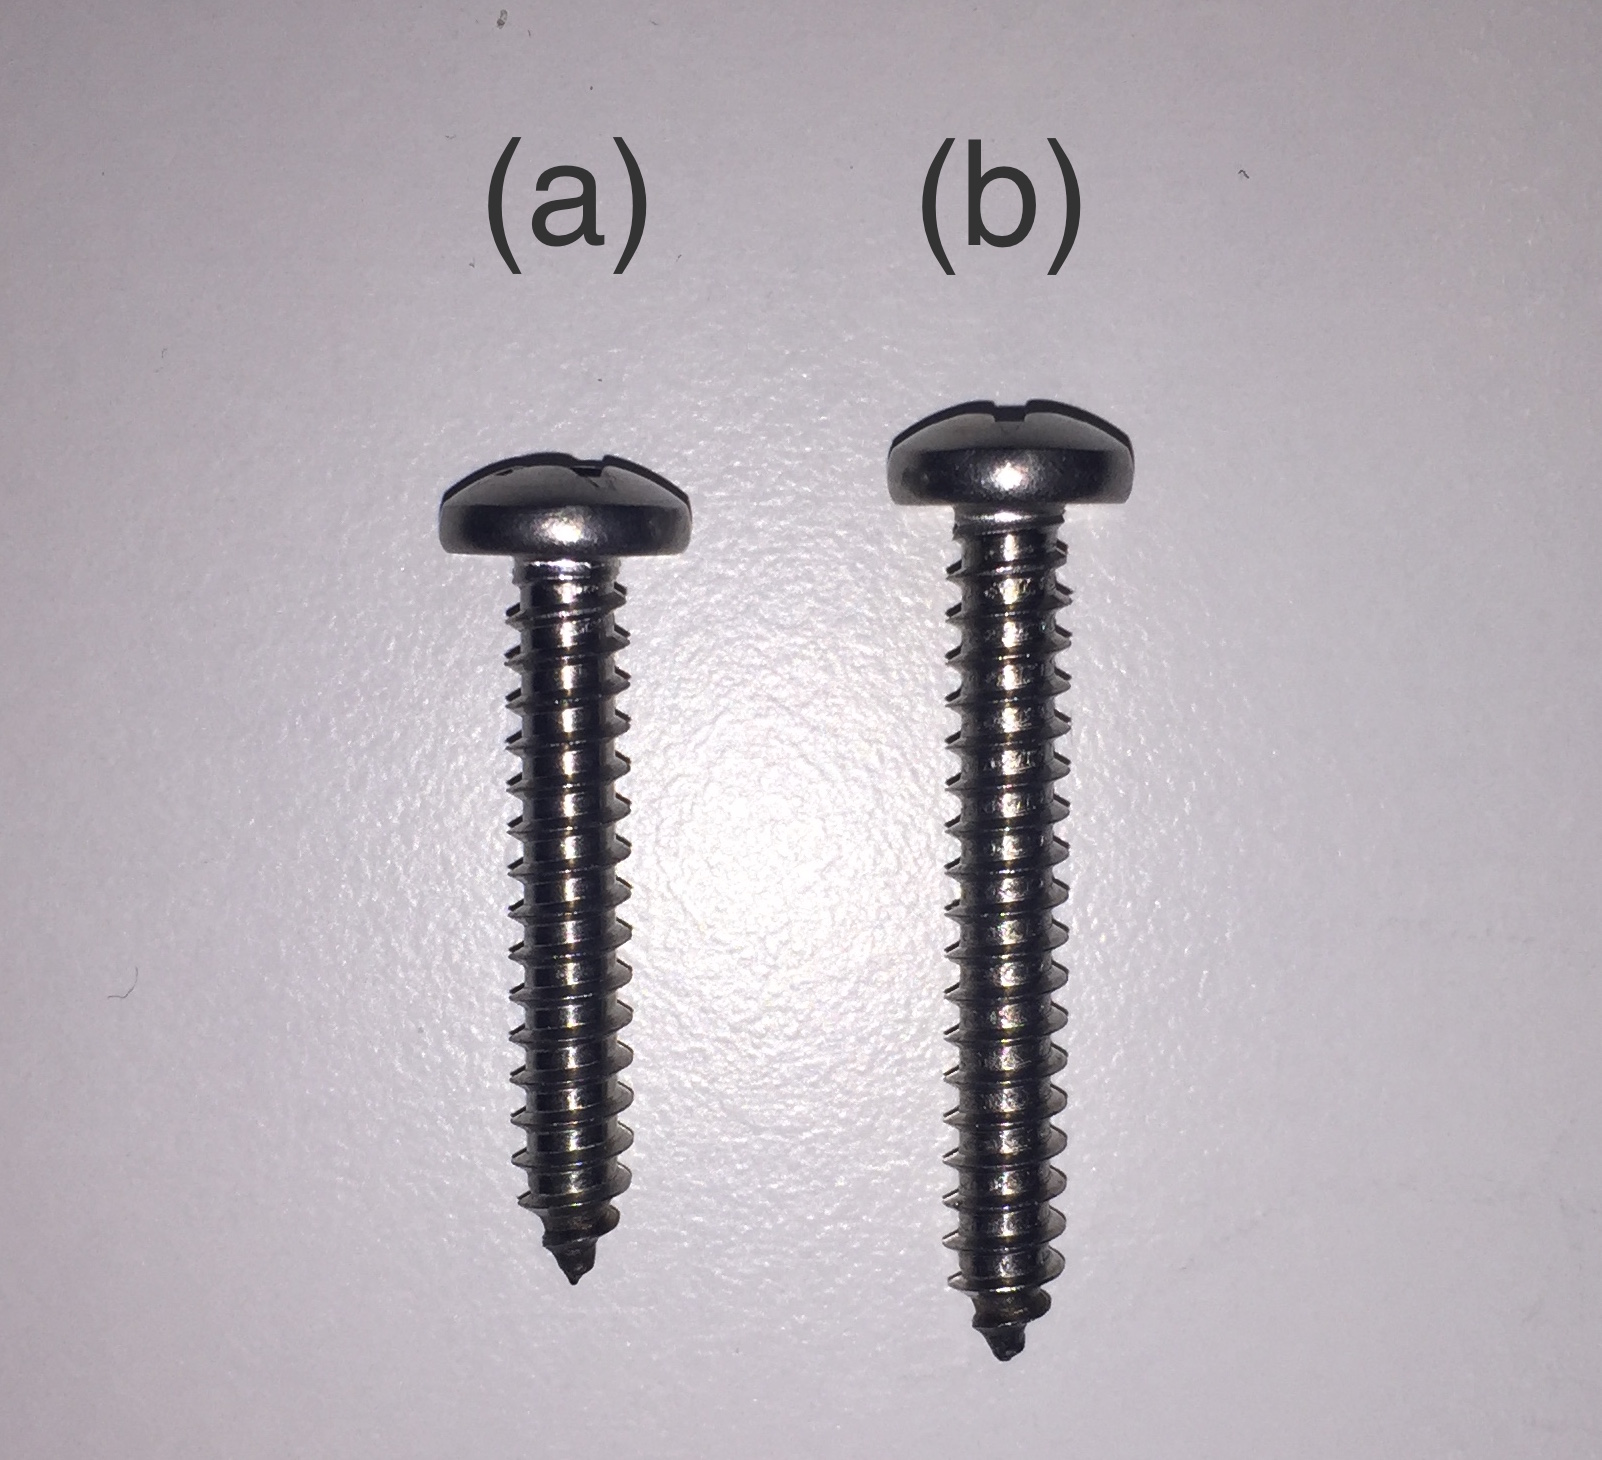
\includegraphics[width=0.5\textwidth]{similar_small_parts}
\caption{Screw (a) is identical to screw (b) except that screw (a) is 6mm shorter than screw (b). An overhead light shines on the 2 screws. The reflection changes the natural color of their surface.}
\label{fig:similar_small_parts}
\end{figure}

Aircraft fasteners are metalic and have a shiny surface. The light reflection off the fastener surface disturbs the natural surface color as shown in figure \ref{fig:similar_small_parts}, and may hide important features. Furthermore, the effect of the light reflection depends on the direction of the light, which may cause variance between images of a single small part.

Unlike cases where the background can provide information, the background is non-informative to the classification of small parts. Additionally, exposure to a regular lighting condition, like an overhead light in a room, causes the fasteners to cast a shadow on their background. A fastener shadow is not a discriminative feature. Both the background and the fastener shadow are a source of noise for the classifier.

\subsection{Real and Synthetic Images}
To automatically classify small parts, we build a convolutional neural network that is trained on both \textbf{real images} and \textbf{synthetic images}. We define real images as the natural images of the small parts, taken using a camera. Synthetic images, on the other hand, are artifically created images. They are 2-dimensional renditions of \textbf{3d models} of small parts. To generate synthetic images, we must create a \textbf{synthetic scene}: an artifical environment created in 3D modeling software. Figure \ref{fig:synthetic_scene} shows an example of a synthetic scene. A 3d model is placed in a synthetic scene in 3D modeling software. The software renders a 2D image of the environment to create a synthetic scene.

The real and synthetic images should capture the small parts and their corresponding 3D models from different angles and in different positions. To do so, we apply \textbf{transformations} to the small parts and 3D models. There are two types of trnasformations: \textbf{translation} to change the position of the target object, and \textbf{rotation} to change the angle. Each transformation has a range. This prevents the target objects from being translated or rotated away from the camera view.

\begin{figure}[h]
\centering
  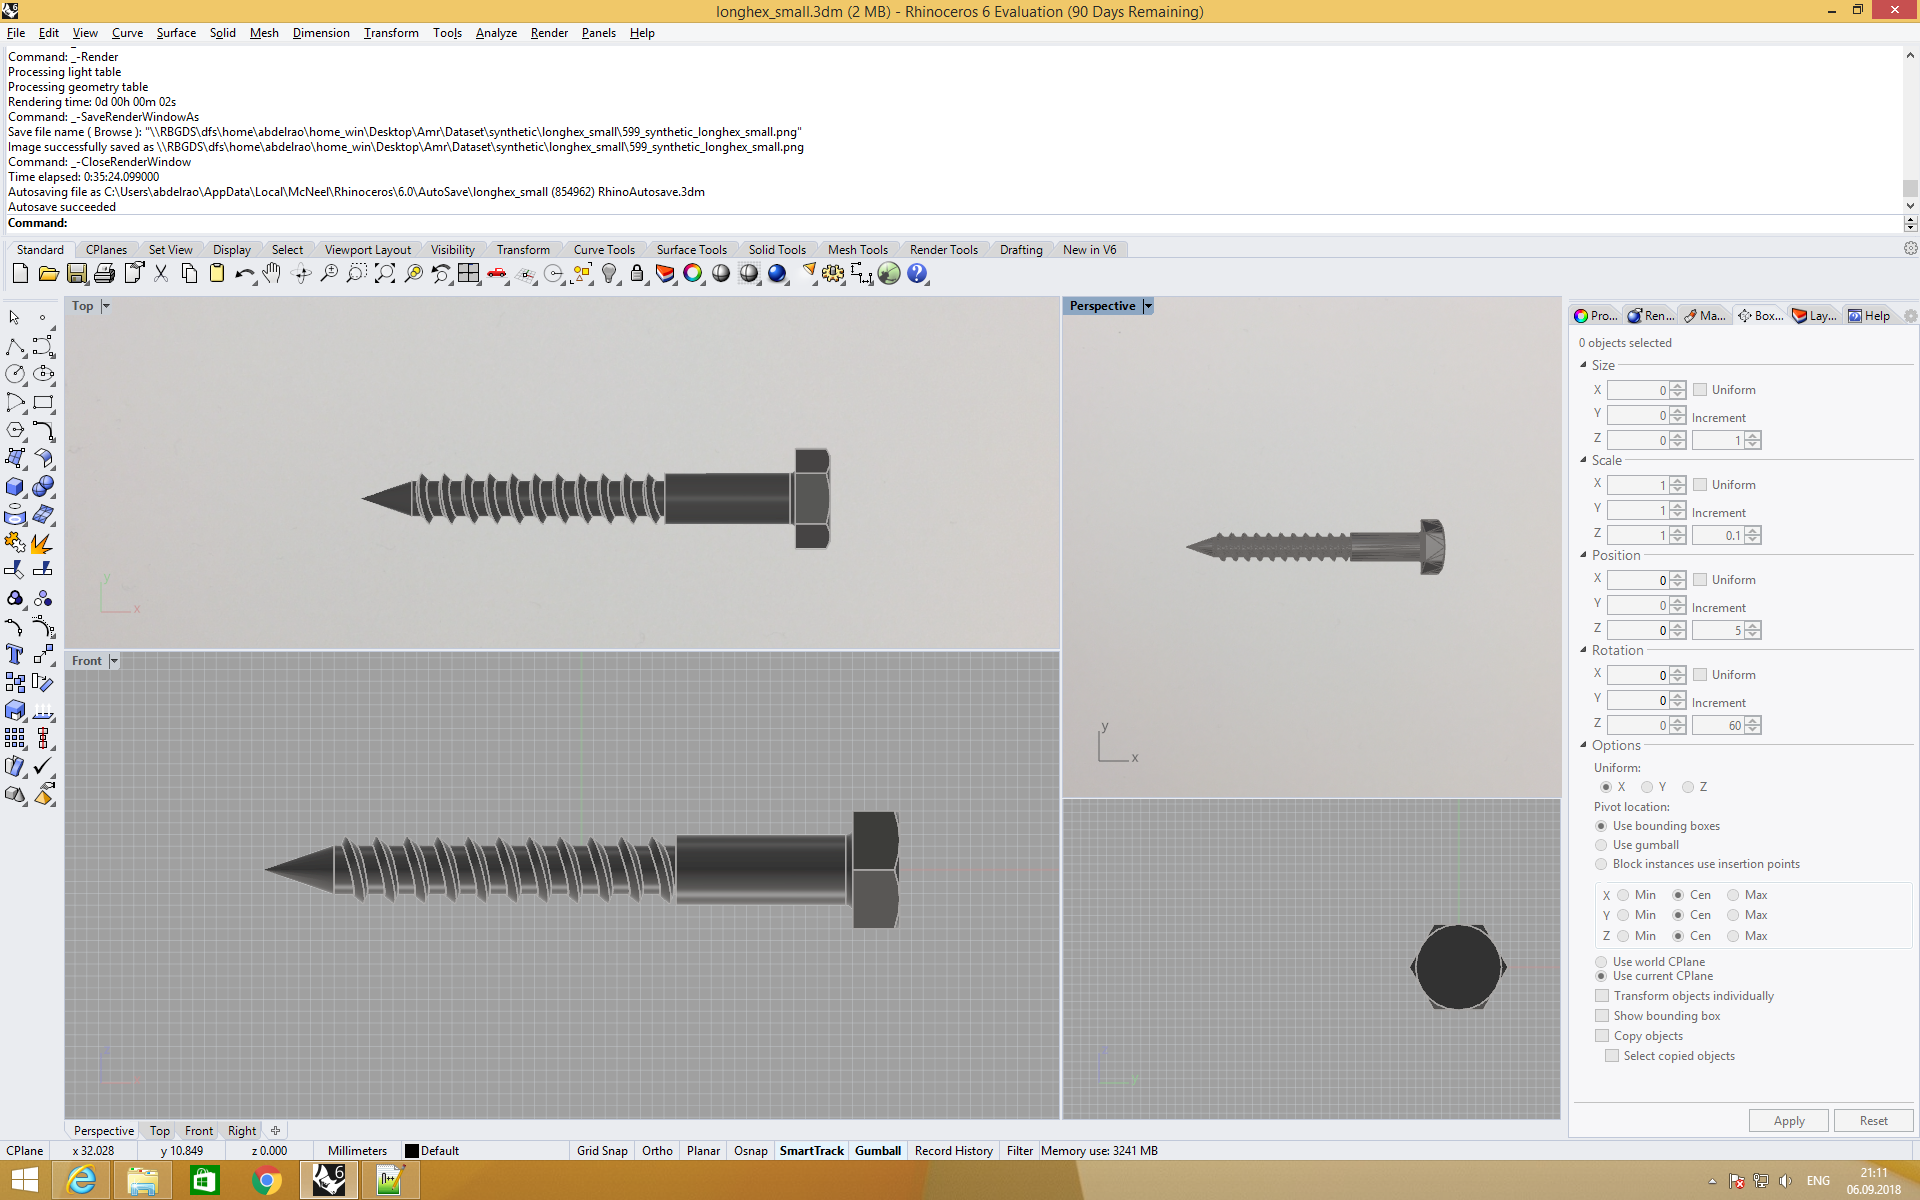
\includegraphics[width=\textwidth]{rhino_screenshot}
\caption{Synthetic scene in Rhino. The 3D model rests horizontally on a backlit plane to mimic the environment of the real setup. Sections (a) and (b) of the image depict the top view of the scene.}
\label{fig:synthetic_scene}
\end{figure}
